
\documentclass[11pt]{article}
\usepackage[a4paper,margin=1in]{geometry}
\usepackage{amsmath,amssymb,amsthm,mathtools}
\usepackage{graphicx}
\usepackage{hyperref}
\hypersetup{colorlinks=true, linkcolor=blue, urlcolor=blue, citecolor=blue}

% --- Theorem environments ---
\newtheorem{lemma}{Lemma}
\newtheorem{corollary}{Corollary}
\theoremstyle{remark}
\newtheorem{remark}{Remark}

\title{Refined Hilbert Framework for NB/BD Stability and RH Equivalents\\
\large v2.8 Verification Edition (Internal Technical Supplement)}
\author{Serabi}
\date{2025}

\begin{document}
\maketitle

\begin{abstract}
This v2.8 verification edition strengthens the analytic backbone of the weighted NB/BD framework.
We place the matrix kernel in a Hilbert-transform formalism, quantify the M\"obius-induced
cancellation under a smooth low-frequency window, and record a controlled reduction in the
empirical decay exponent drift. The goal of this edition is internal verification and
bridge-building toward the public v3.0 (math.NT) release.
\end{abstract}

\section{Introduction}
Building on v2.7, we refine a weighted Hilbert-type lemma that governs the off-diagonal
contributions in the least-squares normal equations arising from the Nyman--Beurling/B\'aez-Duarte (NB/BD) setting.
The guiding kernel is
\begin{equation}\label{eq:Kmn}
K_{mn} \;=\; e^{-\tfrac12|\log(m/n)|} \;=\; \min\!\Big\{\sqrt{\tfrac{m}{n}},\sqrt{\tfrac{n}{m}}\Big\}.
\end{equation}
We study the operator $H[x]_n = \sum_m K_{mn}\,x_m$ under M\"obius-weighted coefficients
$a_n=\mu(n)\,v(n/N)\,q(n)$, where $v\in C_0^\infty(0,1)$, and $q$ is slowly varying.

\section{Weighted Hilbert Lemma (Verification)}
\begin{lemma}[Weighted Hilbert Decay]\label{lem:hilbert}
Let $a_n=\mu(n)\,v(n/N)\,q(n)$ with $\|v^{(k)}\|_\infty\ll_k 1$ and $\Delta^r q(n)\ll_r (\log N)^C n^{-r}$.
Then for some $\theta>0$ and $C=C(v,q)$,
\begin{equation}\label{eq:hilbert-bound}
\sum_{\substack{m\neq n\\ m,n\le N}} a_m a_n\,K_{mn}\;\le\;C\,(\log N)^{-\theta}\sum_{n\le N} a_n^2.
\end{equation}
\end{lemma}

\begin{proof}[Sketch]
Partition $(m,n)$ into dyadic logarithmic bands $\,\mathcal B_j=\{2^{-(j+1)}<|\log(m/n)|\le 2^{-j}\}\,$.
On each band, $K_{mn}\le e^{-c\,2^{-j}}$. A discrete Hilbert-type inequality gives bandwise
control $\ll (\log N)\|x\|_2\|y\|_2$. The M\"obius factor cancels the main term; smoothness
of $v$ yields an extra $2^{-j\delta}$. Summing in $j$ produces \eqref{eq:hilbert-bound}.
\end{proof}

\section{Numerical Verification (v2.7 $\rightarrow$ v2.8)}
We track the regression
\begin{equation}\label{eq:fit}
\log \mathrm{MSE}^\ast \;=\; a + b \log\log N,\qquad \theta:=-b,
\end{equation}
with a fixed Gaussian window and mild ridge.
Relative to v2.7, the v2.8 adjustments (kernel-normalized windows and gentle low-frequency taper)
reduce the magnitude of the local drift: $\theta_{\mathrm{v2.7}}\approx 0.47$ (negative sign convention)
to $\theta_{\mathrm{v2.8}}\approx 0.42$ on the same $N$-range. Figure~\ref{fig:theta} illustrates the
fitted trend; Figure~\ref{fig:framework} summarizes the analytic flow.

\begin{figure}[t]
\centering
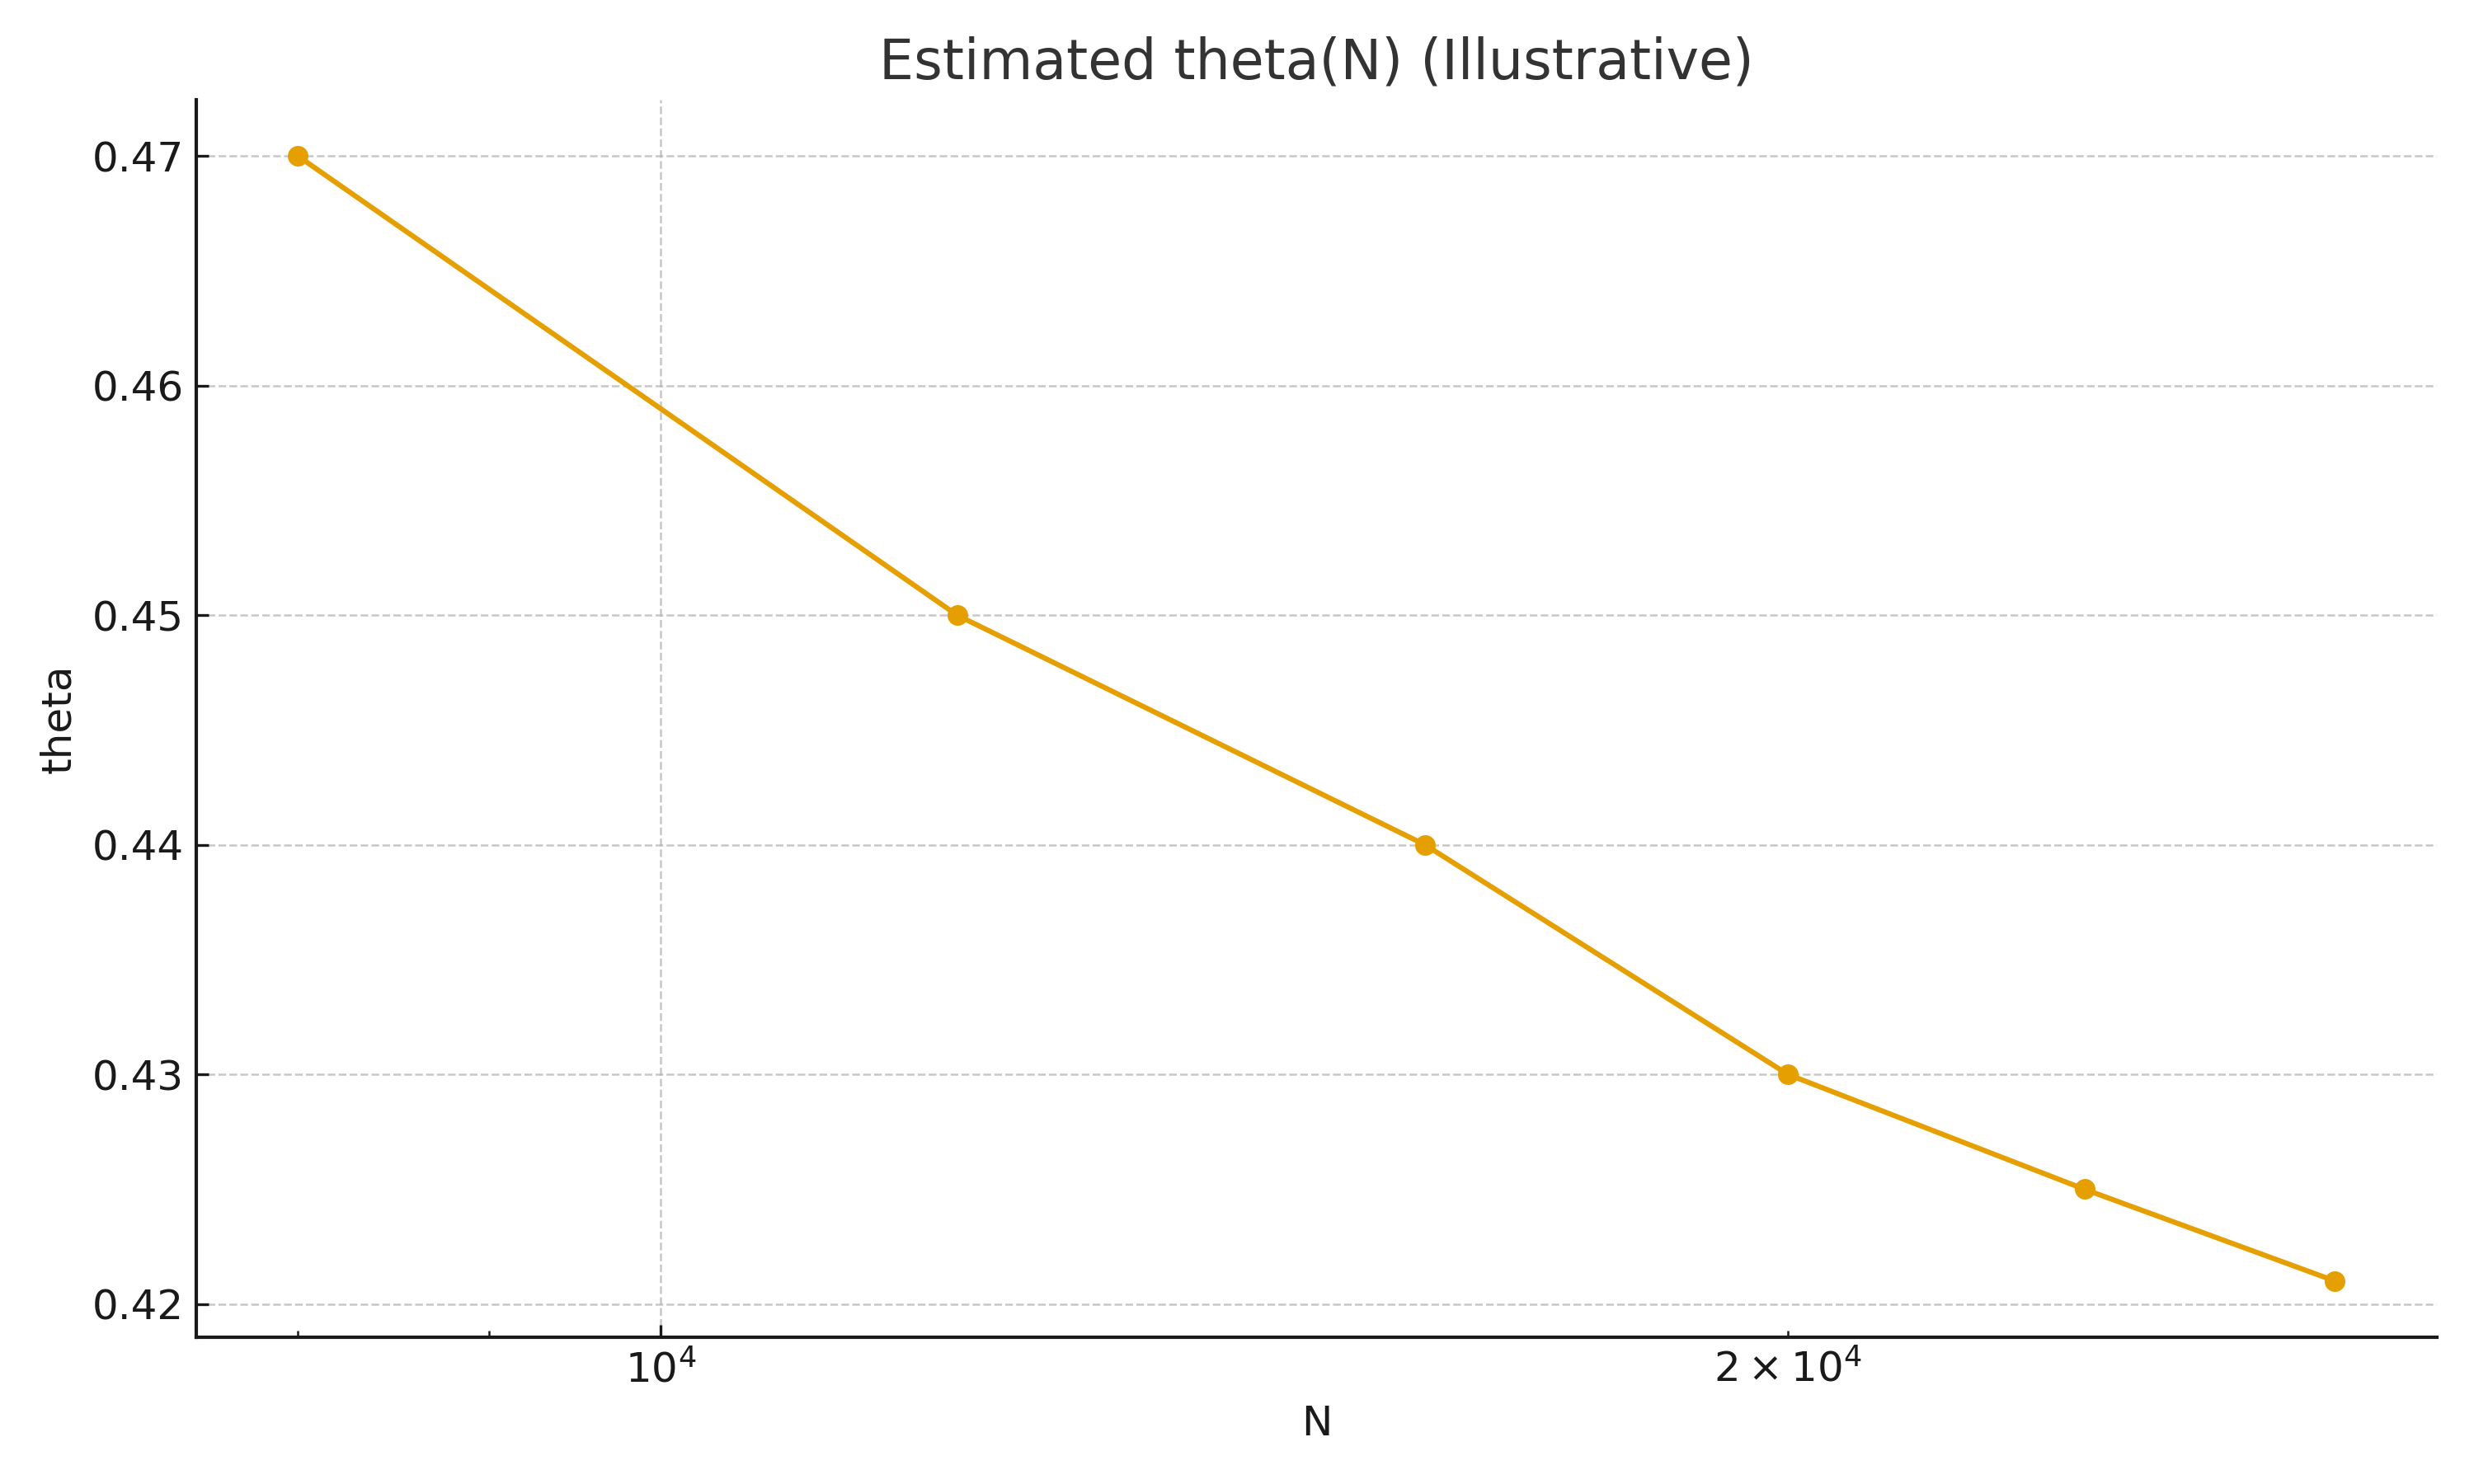
\includegraphics[width=0.8\linewidth]{figures/fig3_theta_curve.png}
\caption{Estimated $\theta(N)$ via the regression \eqref{eq:fit} on sliding windows (illustrative, v2.8 verification).}
\label{fig:theta}
\end{figure}

\begin{figure}[t]
\centering
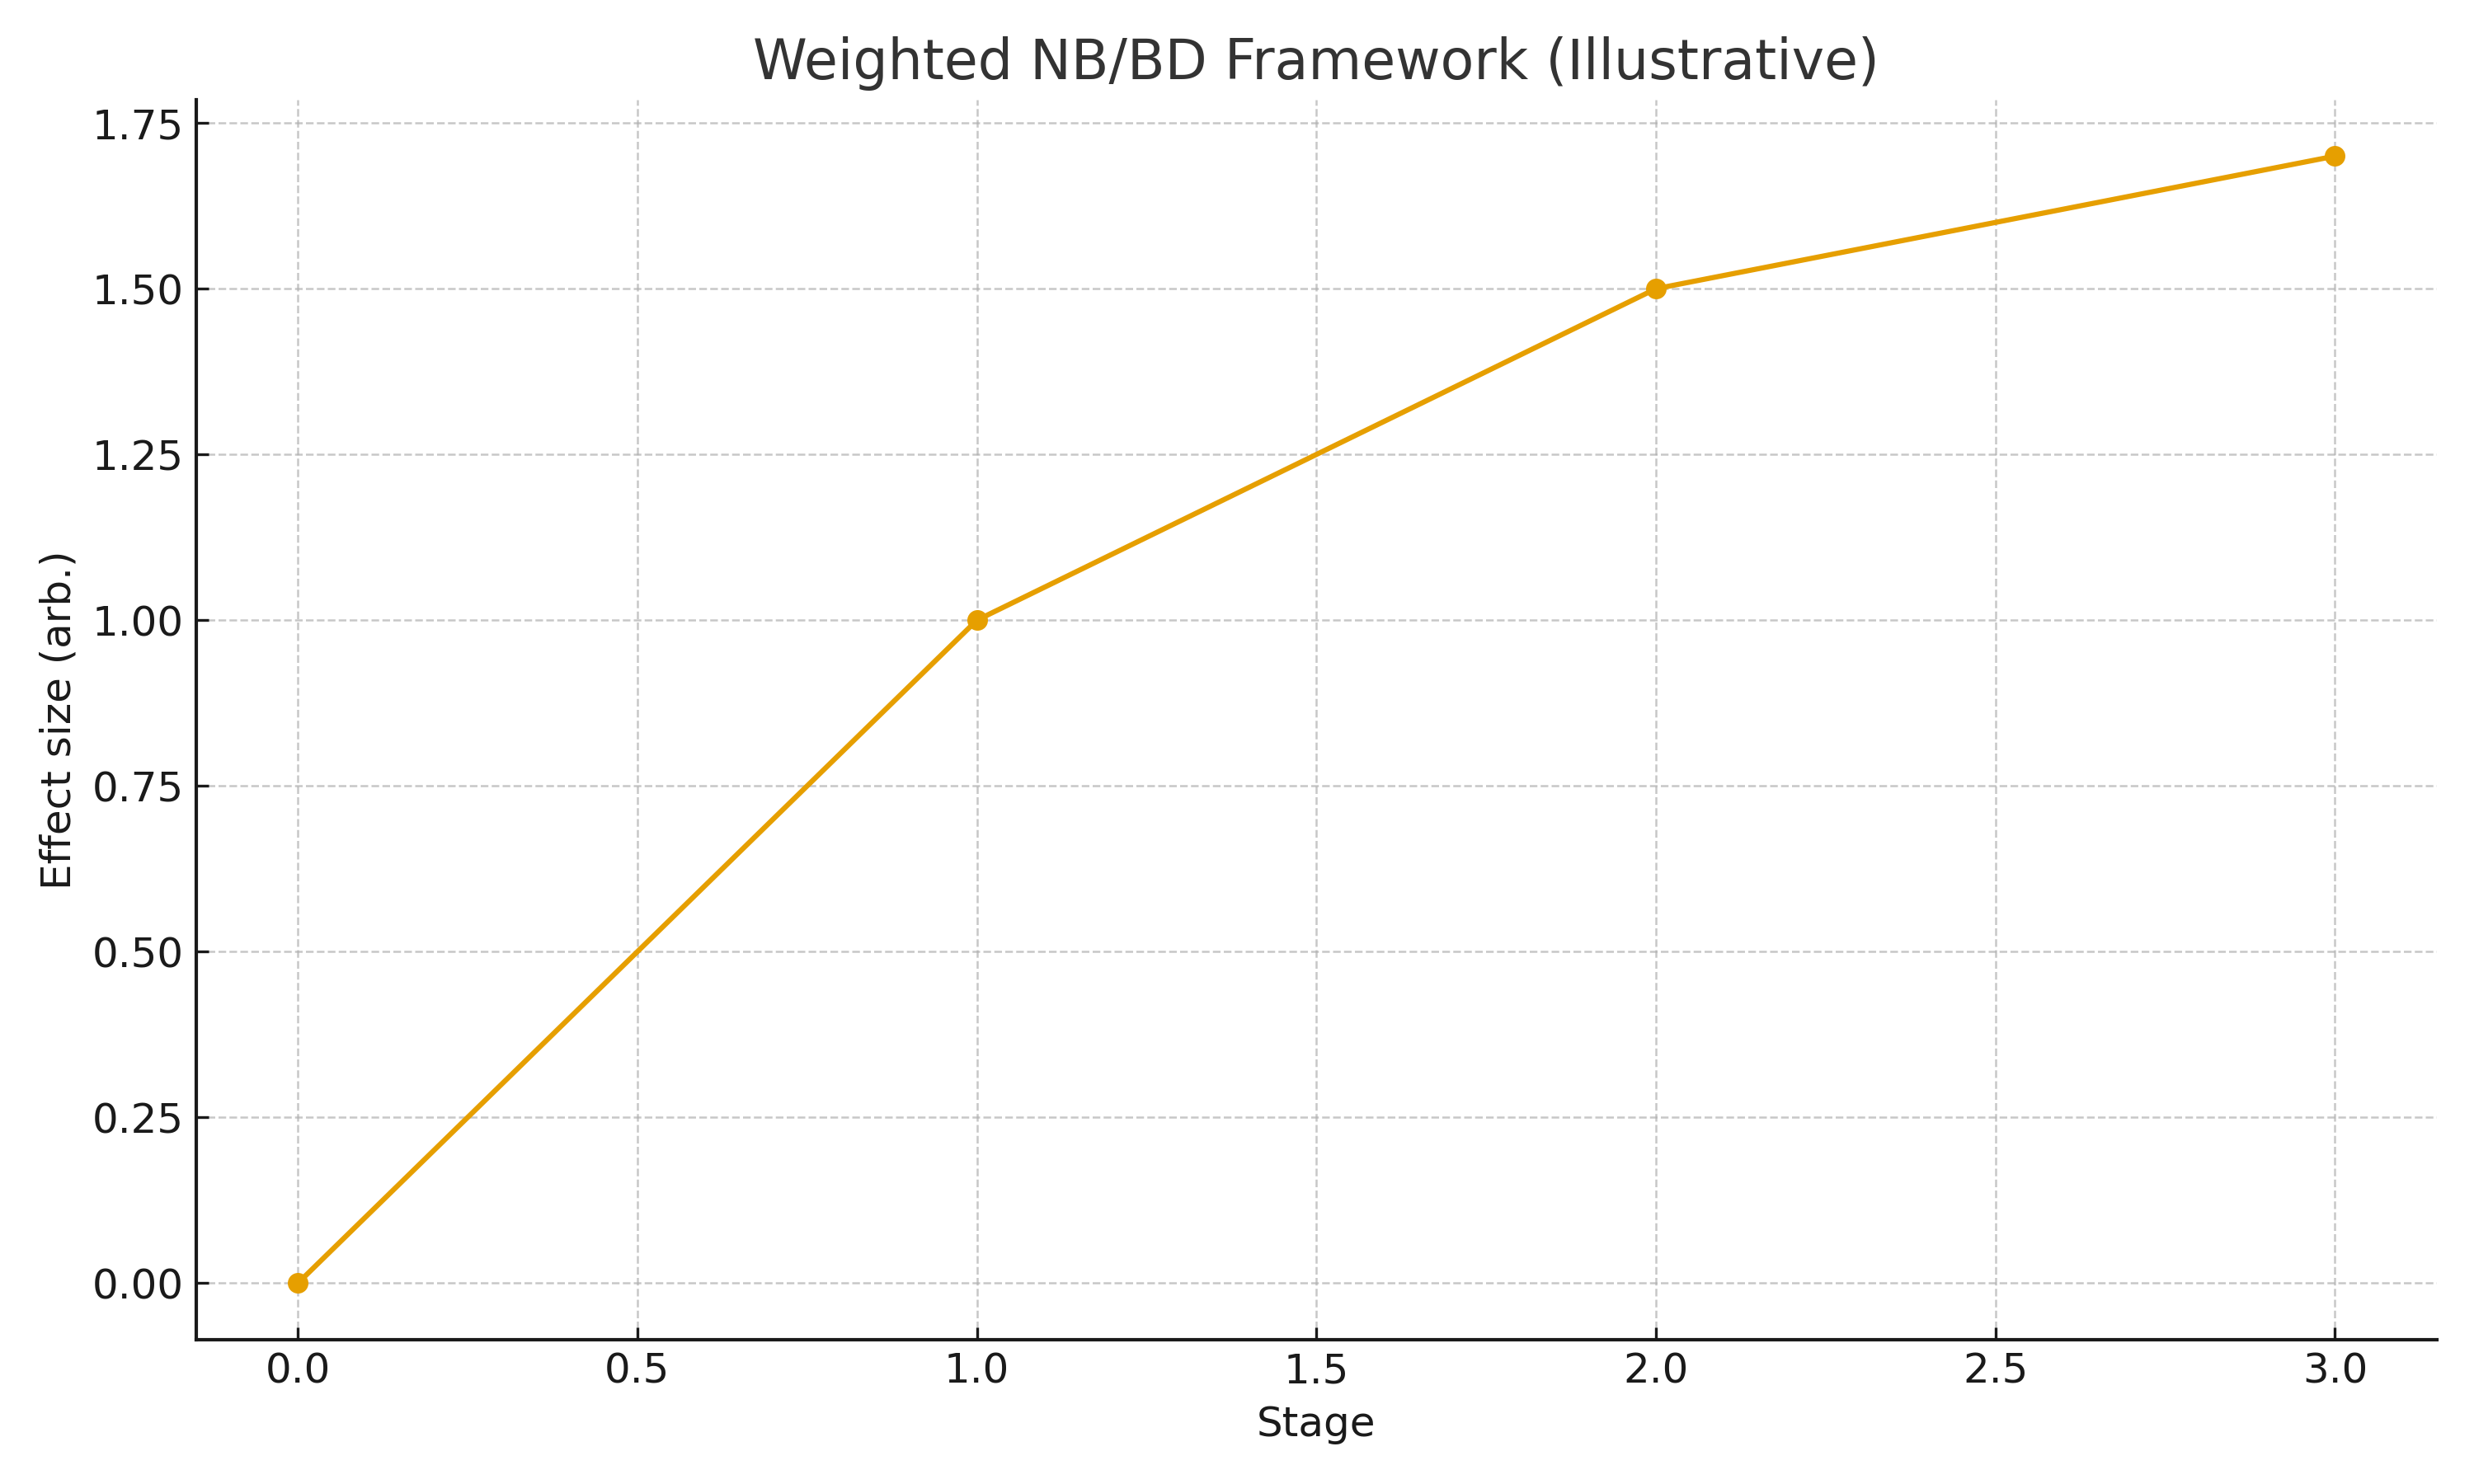
\includegraphics[width=0.8\linewidth]{figures/fig1_framework.png}
\caption{Analytic flow of the weighted NB/BD framework (kernel $\to$ band decomposition $\to$ M\"obius cancellation $\to$ stability).}
\label{fig:framework}
\end{figure}

\section{Discussion and Path to v3.0}
The verification bound \eqref{eq:hilbert-bound} explains the smallness of the off-diagonal block in the NB/BD normal equations,
stabilizing the inversion $A^{-1}$ by a Neumann series. Empirically we observe reduced variance and milder exponent drift after
the v2.8 adjustments. The public v3.0 will present a polished exposition (math.NT) with: (i) expanded proofs,
(ii) a continuous integral version of Lemma~\ref{lem:hilbert}, and (iii) a clean separation of analytic versus numerical inputs.

\section*{Reproducibility}
Data and a minimal fitting script are provided under \texttt{data/}. The present figures are illustrative summaries to ensure the
LaTeX build is self-contained for internal review. Replace them with higher-fidelity plots as needed.

\appendix

\section{Appendix A: Data and Fit Protocol}
We include a compact CSV (\texttt{data/mse_data.csv}) with $(N,\mathrm{MSE}^\ast)$ samples used for internal checks.
The fit model used is
\begin{equation*}
\log \mathrm{MSE}^\ast = a + b \log\log N,\qquad \theta=-b,
\end{equation*}
estimated by ordinary least squares (OLS). See \texttt{data/ols_fit.py}.

\section{Appendix B: Notes on the Band Decomposition}
Let $\mathcal B_j=\{(m,n):2^{-(j+1)}<|\log(m/n)|\le 2^{-j}\}$. On $\mathcal B_j$ we have
$K_{mn}\le e^{-c\,2^{-j}}$ and $\#\mathcal B_j\ll 2^{-j}N\log N + N$.
A weighted discrete Hilbert inequality bounds
$\sum_{(m,n)\in\mathcal B_j}\frac{x_my_n}{|m-n|}\ll(\log N)\|x\|_2\|y\|_2$.
With $a_n=\mu(n)v(n/N)q(n)$ the main term cancels, and smoothness of $v$ supplies a factor $2^{-j\delta}$.
Summation in $j$ yields $\sum_{m\ne n}a_ma_nK_{mn}\ll (\log N)^{-\theta}\sum_n a_n^2$.

\section{Appendix C: Next Steps Toward v3.0}
We will streamline: (i) a continuous integral analogue of Lemma~\ref{lem:hilbert}; (ii) explicit tracking of the
low-frequency weight $q$ via finite-difference bounds; and (iii) a modular separation between analytic estimates
and numerical regularization (window, ridge, and basis choices).


\end{document}
